%!TEX root = ../../thesis.tex

\section{\eniric{}: Extended \nir{} information content}
\label{sec:eniric}
Here the software developed to compute the {RV} precisions is presented.
It is an extension of the code used for the calculations of~\citet{figueira_radial_2016}, hence ``extended'' in the name.
This section documents the vast improvements (optimizations and extensions) made to the software.
Changes made that affect the derived {RV} precision attained are specifically documented in detail, with the relative precision changes provided.
This work resulted in a submission of a publication\footnote{Available at \href{http://joss.theoj.org/papers/384bfc031df47ecef2d88328f63e5479}{http://joss.theoj.org/papers/384bfc031df47ecef2d88328f63e5479}} to \emph{The Journal of Open Source Software}\footnote{\href{http://joss.theoj.org/}{joss.theoj.org/}.} (JOSS) (Neal and Figueira 2019 \emph{almost accepted}) with the source code openly available on \href{Github}{https://github.com/jason-neal/eniric}.


\subsection{Automated testing}
\label{subsec:automated_testing}
Before the changes to the software are detailed, a note about software testing.
Automated software testing is an important practise to ensure that the code written is correct, and that new changes to not break the previously written code.
This practice is crucial in computer science and professional software engineering but seldom encouraged or practised in scientific programming~\citep{storer_bridging_2017}.
It is however starting to becoming increasingly encouraged as part of the movement towards open and reproducible science.

After inheriting the code-base from~\citet{figueira_radial_2016}, software tests were added for a number of purposes: to learn and explore the code-base, to check and test the original functionality, and to identify if any changes implemented break the original functionality.
Version control practises were used to incrementally add small separate changes to the code base at a time, regularly testing in a continuous integration manor.
This is done by sending the code-base to a repository\footnote{Public or private.} on Github\footnote{\href{https://bitbucket.org}{Bitbucket} and \href{https://gitlab.com}{GitLab} are other popular options.}.
Automated tools and services then forward the project to testing, code style checking, or other continuous-integration services (e.g.\ \href{https://travis-ci.com}{Travis-CI}) which either run the automated tests, or other checks on each new change.
The public Travis-CI record of the test for \eniric{} can be found at \href{https://travis-ci.org/jason-neal/eniric}{https://travis-ci.org/jason-neal/eniric}.

This process was valuable in preventing the introduction of errors, but also in identifying and errors in the~\citep{figueira_radial_2016} results which are outlined in \cref{subsec:condition_two_bug}.
Based on this experience it is a practise that is highly recommend for scientific programming.


\subsection{Performance}
\label{subsec:code_performance}
The software performance is one aspect that was addressed in the upgrades.
The original code used in~\citet{figueira_radial_2016} was very slow, taking around two hours per parameter combination.
This led to multiple weeks worth of processing time required to compute the {RV} precision for the original paper (180 combinations).
The latest implementation of \eniric{} can compute all 180 combinations in less than two hours.

The major performance bottleneck was identified in the convolution stage.
Stating with a \numpy{} array containing the spectrum the algorithm looped though each pixel in the spectrum, selecting a suitable window around the given pixel with a \emph{comprehension list}\footnote{Example usage can be found \href{https://docs.python.org/3/tutorial/datastructures.html\#list-comprehensions}{here}.}.
The output is a list\footnote{A list is a native Python data structure.} which was turned back into a \numpy{} array, eventually summed and then appended to a new list.
This list was once again converted into \numpy{} array.
The main performance issue is a Python implementation detail to do with a type checking overhead when converting between \numpy{} and native data types.
These conversions were performed 2--3 times for every pixel in the large spectral arrays of order \({10}^{4}\) pixels.

Remaining entirely in the fast compiled \numpy{} code and not changing data types a performance gain of around 250\(\times\)\,X was achieved.
This is done by using boolean masks instead of comprehension lists and pre-allocating a \numpy{} array to store the results a itself.

The convolution computation of individual pixels is an ``embarrassingly parallel''\footnote{\href{https://en.wikipedia.org/wiki/Embarrassingly\_parallel}{https://en.wikipedia.org/wiki/Embarrassingly\_parallel}.} problem.
What this means is that convolution result for pixel $i+1$ does not depend on the convolution result obtained of pixel $i$, each can be computed independently.
Therefore, parallel processing was also added into the convolution to further improve the performance, roughly dividing the convolution time by the number of processors used.

As the convolution step is the main bottleneck, caching of the convolution results was included using the \href{https://joblib.readthedocs.io}{Joblib} package.
Caching the convolution function stores the input parameters and the convolution result together.
If the same input parameters are passed to the convolution function again, it fetches the computed results from memory, rather than recomputing the time intensive convolutions.
This avoids unnecessary wasted computation time computing the same convolution results, improving the performance of repeated runs of the software.

The \pyastronomy{} package has a ``slow'' version of the rotational convolution, which has a wavelength dependent kernel as done here.
They also provide ``fast'' convolution kernels that used fixed kernel, taking the central wavelength value.
These are significantly faster but are only valid for very short wavelength regions, in which the kernels do not significantly change.
They are not deemed suitable for use in this work due to the large wavelength span of spectroscopic bands and the wavelength dependant spacing of the spectra considered here.
A comparison of the performance between the \pyastronomy{} convolutions and the convolutions implemented in \eniric{} and used here are provided in a \emph{Jupyter} notebook in the Github repository of ``eniric''\footnote{\href{https://github.com/jason-neal/eniric/blob/master/docs/Notebooks/Convolution_speeds.ipynb}{https://github.com/jason-neal/eniric/blob/master/docs/Notebooks/Convolution\_speeds.ipynb}.}, basically they fall in between the ``fast'' and ``slow'' implementation of \pyastronomy{}.


\subsection{Model extension}
\label{subsec:eniric_model_extesion}
The original software hard-coded the range of 180 model combinations computed, specifically by identifying the spectra by their spectral type and setting the \snr{} scaling values.
These combinations were the four model spectra (M0, M3, M6, M9), three resolutions (60\,000, 80\,000, 100\,000), three \Vsini{} values (1.0, 5.0, 10.0\kmps{}) and the five spectral bands (\emph{Z}, \emph{Y}, \emph{J}, \emph{H}, \emph{K}).

The software was extended to be able to load and prepare any spectrum from the {PHOENIX-ACES} spectral library provided the four identifying parameters [\Teff, \Logg, \feh{}, \alphafe{}].
This allows for any spectra of current or future interest to be quickly analysed, matching any of parameters in \cref{tab:phoenix}.
The instrumental resolution, \(R\), and rotation velocity \Vsini{} were also extended to any suitable value, not restricted to only three values each.
The \nir{} wavelength bands are still configured to the same wavelength regions but are able to be extended by the user, either over-writing the current band limits, or defining new bands with custom wavelength limits.
For example, in \cref{tab:numerical_gradients} bands (and corresponding wavelengths) with labels \({\rm VIS}\), \(\rm {CARM}_{VIS}\), \(\rm {NIR}\) and \(\rm {CARM}_{NIR}\) are shown which represent the visible and \nir{} wavelengths and the corresponding coverage of the {CARMENES} spectrograph in each.
This allows for increased flexibility in using \eniric{}, for instance tailoring the calculation to a specific instrument with a known or theoretical resolution (see \cref{sec:spirou_nirps_etc}), but opens up essentially an infinite possible combination of spectral parameters (with an infinite compute time).

A further extension was made to also allow for the use of the {BT-Settl} ({CIFIST2011\_2015}) synthetic spectra.
Allowing for a comparison of RV precisions between different models.
Like the {PHOENIX-ACES} models the {BT-Settl} spectra undergo a conversion from an energy flux to photon counts.
The incorporation of any model from the {PHOENIX-ACES} and {BT-Settl} libraries with only the four model parameters is performed simply using the ``grid tools'' module from the Starfish package\citep{czekala_constructing_2015}.
to similar treatment to the {PHOENIX-ACES} models, being converted to photon counts.

A command line application is now available with \eniric{}, which will load spectra and calculate RV precision for all combinations of valid input parameters.
Examples of use are given in \cref{app:nir_prec_amendment}, specifically all parameter combinations from~\citep{figueira_radial_2016} can be performed using \cref{lst:commandline_incantation}.


\section{Numerical Gradient}
\label{sec:numerical_gradient}
One of the key insights from \cref{eqn:optimal_weight,eqn:dv_rms} is that the radial velocity precision is inversely proportional gradient of the spectra.
In numerically computing the {RV} precision, the result is dependent on the numerical method used to compute the gradient.
In the original code used in~\citet{figueira_radial_2016} the gradient is approximated using the forward finite difference {FFD} method.
In \eniric{} the method for computing the gradient is changed to the \npgradient{} function from the \numpy{} package.
This uses more advanced numerical methods to compute a more precise gradient.
A comparison between both gradient methods and the affect on the precisions result are presented here.

The simplest way to calculate the derivative is using finite difference methods~\citep{quarteroni_numerical_2000}.
These arise from the Newton's definition of the derivative for a continuous function \(f(x)\) which should be familiar from introductory calculus:
\[f'(x) = \lim_{h \to 0} \frac{f(x+h)-f(x)}{h}~.\]

The three common varieties of the finite difference are,
\begin{equation}
{FFD} = \frac{f(x+h)-f(x)}{h}, {CFD}=\frac{f(x+\frac{1}{2}h)-f(x-\frac{1}{2}h)}{h}, {BFD}=\frac{f(x)-f(x-h)}{h}\,,
\end{equation}
and are called the forwards ({FFD}), central ({CFD}), and backwards ({BFD}) finite differences respectively.
The order of uncertainty on the {FFD}/{BFD} methods is \(\mathcal{O}(h)\) while for the {CFD} it is \(\mathcal{O}({h}^{2})\)~\citep{quarteroni_numerical_2000}.
As the wavelength spacing between samples/pixels (h) is small the {CFD} will be more precise value for the gradient at each pixel.

In this case \(h\) is the difference in wavelength between the two pixels considered.
In the {FFD} case the gradient at pixel \(i\) becomes:
\begin{equation}
\frac{\partial {A}_{0}(i)}{\partial\lambda(i)} = \frac{{A}_{0}(i+1) - {A}_{0}(i)}{\lambda(i+1)-\lambda(i)}, \hspace{2em} 1 \leq i \leq n-1.
\label{eqn:ffd_precision}
\end{equation}
At each pixel the numerical derivative is evaluated to be the average slope between itself and the following pixel and is an approximation to the derivative.
This only extends to \(i= n-1\), where \(n\) is the number of points in the spectrum, and the last pixel is dropped from the {RV} calculation.
This is important in the case of Condition~\#2 (\cref{eqn:mask2}) from~\citet{figueira_radial_2016}.


The \npgradient{}\footnote{Documentation available at \href{https://docs.scipy.org/doc/numpy/reference/generated/numpy.gradient.html\#id1 }{https://docs.scipy.org/doc/numpy/reference/generated/numpy.gradient.html\#id1}.} function contains a more advanced numerical method to calculate the derivative.
It uses a \textit{compact difference} method~\citep{quarteroni_numerical_2000} which expands the finite differences using a Taylor expansion and then selects coefficients to minimize the \textit{consistency error}.
From the \numpy{} documentation the consistency error here is \[\eta_i = \partial{f(x_i)}/\partial{x} -  [\alpha f(x_i) + \beta f(x_i +h_d) + \gamma f(x_i - h_s)],\] where \(h_s\) and \(h_d\) are the spacing to the left and right of \(i\) respectively.
With Taylor expansion this turns into solving a linear system of equations:
\[\begin{cases}
\alpha + \beta + \gamma = 0\\
-\beta {h_d} + \gamma {h_s} = 1\\
\beta {h_{d}}^{2} + \gamma {h_{s}}^{2} = 0
\end{cases}
\]
which result in the approximation of the gradient of the central values to be

\[\frac{\partial{f(x_i)}}{\partial{x}} = \frac{{h_{s}}^{2}f\left(x_{i} + {h_{d}}\right) + \left({h_{d}}^{2} - {h_{s}}^{2}\right)f\left(x_{i}\right) - {h_{d}}^{2}f\left(x_{i}-{h_{s}}\right)} {{h_{s}}{h_{d}}\left({h_{d}} + {h_{s}}\right)} + \mathcal{O}\left(\frac{h_{d}{h_{s}}^{2} + {h_{s}}{h_{d}}^{2}}{{h_{d}} + {h_{s}}}\right) \label{full_compact_difference}.\]

If the spectrum is evenly spaced ${h_{s}}={h_{d}}$  reduces to the standard second order {CFD} approximation:

\[\frac{\partial{f(x_i)}}{\partial{x}} = \frac{f\left(x_{i+1}\right) - f\left(x_{i-1}\right)}{2h} + \mathcal{O}\left({h}^{2}\right)\]

Applying this to the situation presented here, similar to \cref{eqn:ffd_precision}, results in:
\[\frac{\partial {A}_{0}(i)}{\partial\lambda(i)} = \frac{{\lambda(i-1)}^{2} {A}_{0}(i+1) + ({\lambda(i+1)}^{2}-{\lambda(i-1)}^{2}) {A}_{0}(i) - {\lambda(i+1)}^{2} {A}_{0}(i-1)} {\lambda(i-1)\lambda(i+1)(\lambda(i+1) + \lambda(i-1))}, \hspace{1em} 2 \leq i \leq n-1\]

with an uncertainty of \(\mathcal{O}\left(\frac{\lambda(i+1){\lambda(i-1)}^{2} + \lambda(i-1){\lambda(i+1)}^{2}}{\lambda(i+1) + \lambda(i-1)}\right)\).
As a slight a aside, due to the spectral re-sampling to three pixels per resolution element, the wavelength spacing \(\delta\lambda\) between pixels is a function of \(\lambda\), resolution and sampling choices.

The \npgradient{} function implements central differences for the interior points, accurate to second order, and first order accurate one-sided (forward or backward) differences at the boundaries, computed using the same compact difference procedure.

\begin{figure}
    \centering
    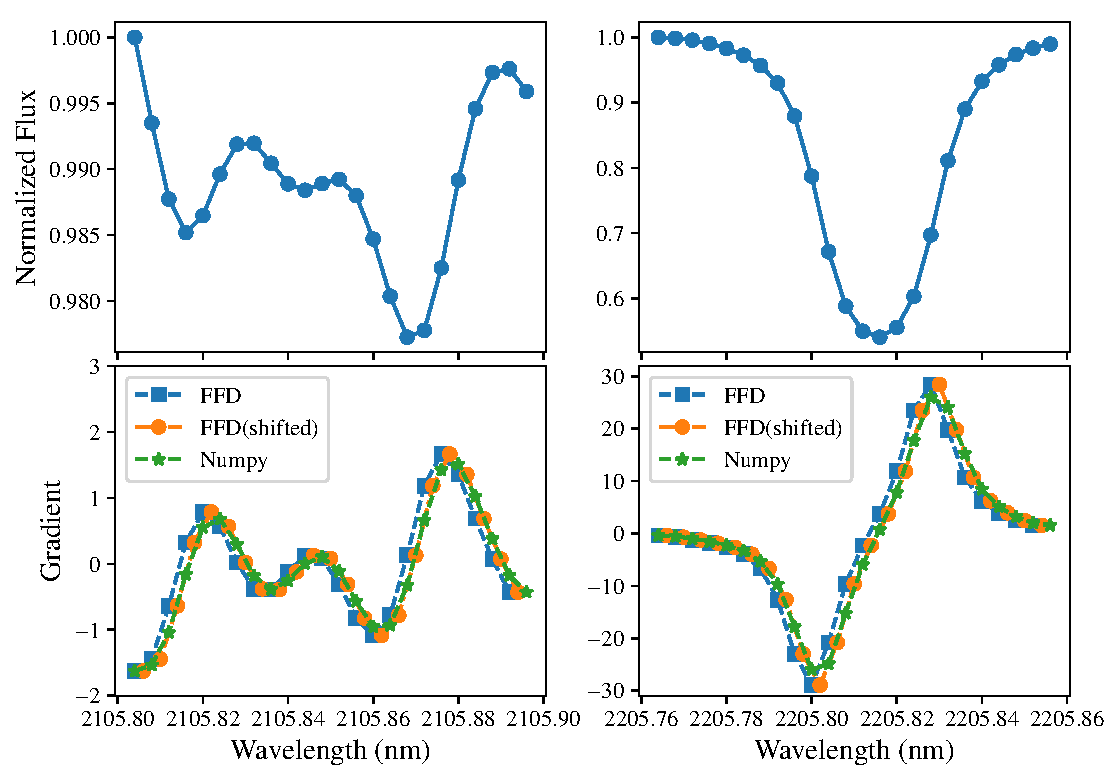
\includegraphics[width=0.85\linewidth]{figures/information-content/spectral_gradients}\\
    \caption[Comparing of numerical gradient alogithms.]{Visualization of the numerical gradient of some spectral lines.
        Top: The two spectral regions of a stellar spectrum the left hand slide contains short lines near the normalized continuum while on the right a single deep absorption line is shown.
        Bottom: The numerical gradients for the spectra shown in the top panels; the original {FFD} method is displayed with \emph{blue squares} while \numpy{} gradient is shown with \emph{green stars}.
        The \emph{orange circles} are the {FFD} version shifted to the mid-points between pixels for illustrative purposes.}
    \label{fig:gradients}
\end{figure}


%!TEX root = ../thesis.tex

\begin{table}
    \centering
    \caption[Affect of numerial gradient.]{The affect of the numerical gradient function on {RV} precision.
        The band label \(\rm VIS\) and \(\rm NIR\) indicate the full visible and \nir{} bands while  \(\rm CARM_{VIS}\)  and \(\rm CARM_{NIR}\) indicate the two wavelength bands of the {CARMENES} spectrograph.
        Column A is the RV precisions calculated using the {FFD} gradient.
        Column B contains the {FFD} gradient method but applied with a wavelength shift of \(\Delta\lambda/2\) in between pixels for this comparison only.
        Column C contains the RV precision calculation using the \npgradient{} function.
        The final two columns give the relative precision change between gradient method A and the other two, as a percentage.
        The {M0} spectra used here had no rotation, or instrument broadening performed and was normalized to a maximum of 1 in each band.
        The values given here are for accessing the relative precision change due to the different gradient methods only.}
    \begin{tabular}{ccccccc}
        \toprule
        %% Band & \(\lambda\) range\_min & wl\_max &  dy/dx   & gradient & Q(dy/dx) & Q(grad) & Q(frac) & {RV}(dy/dx) & {RV}\_adj &    {RV}(grad)    &    {RV}(frac\_grad)    & {RV}(frac\_adj)          \\
        Gradient method &  &  A &   B & C & (B-A)/A & (C-A)/A \\
        &   \(\lambda\) range & FFD & FFD+\(\Delta\lambda/2\) &  Numpy & \(\Delta\delta V\) ratio& \(\Delta\delta V\) ratio\\

        Band  & (\si{\micro\meter})  & \multicolumn{3}{c}{\(\delta V_{rms}\) (\mps{})}  & (\%) & (\%) \\
        \midrule
        VIS & 0.38 -- 0.78 & 16.1 & 16.2 & 16.9  & 0.6 & 4.9\\
        \(\rm CARM_{VIS}\) & 0.52 --  0.96 & 20.9 & 21.0 & 22.0 & 0.3 & 5.2 \\
        Z & 0.83 -- 0.93 & 76.9 & 77.0 & 78.8  & 0.1 & 2.5\\
        Y & 1.00 -- 1.10 & 78.3 & 78.5 & 83.8 & 0.2 & 7.0 \\
        J & 1.17 -- 1.33 & 149.3 & 149.4 & 156.4 & 0.1 & 4.7 \\
        H & 1.50 -- 1.75 & 119.4 & 119.5 & 122.3 & 0.1 & 2.5 \\
        K & 2.07 -- 2.35 & 153.4 & 153.7 & 157.7  & 0.2 & 2.8\\
        \(\rm CARM_{NIR}\) & 0.96 -- 1.71 & 46.1 & 46.2 & 48.0 & 0.1 & 4.2 \\
        NIR & 0.83 -- 2.35 & 36.9 & 36.9 & 38.2 & 0.1 & 3.6  \\
        \bottomrule
    \end{tabular}\label{tab:numerical_gradients}
\end{table}


\cref{fig:gradients} visualizes two small spectral regions with the gradients computed with the original {FFD} and the \npgradient{} methods.
The top panels contain a small section of a simulated spectrum, comprised of three small blended lines, and a large single line respectively.
The derivative of the spectrum for the {FFD} method (blue squares) and \npgradient{} method (green stars) are shown in the bottom panels.
The \emph{orange circles} are the same as the {FFD} method but shifted horizontally to the midpoints between the pixels for which the gradient is calculated at.
This is for illustrative purposes and to assess the affect of this offset when calculating the pixel weights.

There a three notable features observed between gradient methods.
The first, which is expected from the {FFD} formulation is that the {FFD} gradient is offset to the left by half of a pixel.
The second is that when the horizontal offset is adjusted (orange circles) the two gradients lie along the same curve.
Both methods are trying to approximate the real gradient function of the spectrum so it is expected that they should agree.
The most important feature observed in this though is that there is a slight over-estimate of the gradient by the {FFD} method at the peak of each extrema.
The points of highest gradient are always from the {FFD} method (blue/orange).
This is the case for all spectral lines and as the optimal pixel weights are proportional to the gradient squared the {FFD} method will apply slightly higher pixel weights to these values, two points per line in the spectrum.
Therefore, the {FFD} gradient produces a slightly smaller \(\delta V_{\rms}\) error compared to the more precise gradient function.

The numerical differences between to the gradient methods on the relative RV precisions is given in \cref{tab:numerical_gradients}.
The \(\delta V_{\rms}\) is calculated using both gradient methods on a {PHOENIX-ACES} spectrum with \Teff{}=3900\K{}, corresponding to {{M0}} spectral type.
The full theoretical precision is calculated (no telluric masking applied) with no rotational or instrumental broadening and the maximum of the continuum of each band scaled to 1.
In this case the {RV} precisions are not comparable between bands and are only to assess the direct effect of the numerical gradient.
The bands name and the spanned wavelength are given.
The {RV} precision calculated with different gradients are given in columns A, B, C.
A is the original {FFD} method, B is the {FFD} method offset by \(\Delta\lambda\) and C is the \npgradient{}.
The \(\delta V\) ratios are the relative difference in {RV} when changing from method A (the original {FFD}) to methods B and C.

As the pixel weights \cref{eqn:optimal_weight} are proportional to \({\lambda}^{2}\) column B was computed to assess the affect of the slight wavelength offset on the {RV} precision, visible in \cref{fig:gradients}.
\cref{tab:numerical_gradients} shows that wavelength offset of \(\Delta\lambda/2\) contributes 0.1--0.6\% to the RV precision values, an order of magnitude smaller than the change from A to C.
Changing to use the gradient from \numpy{} increases the \(\delta V_{\rms}\) by 2.5--7\%, (decreasing the {RV} precision).
After ruling out the wavelength offset with B, it is assumed that this difference mainly to the over-estimated gradient from the {FFD} method, shown in \cref{fig:gradients}

Changing the method of numerical derivatives will change all the precision values given in the~\citet{figueira_radial_2016}.
This is a small impact on the precision compared to other components of the {RV} precision.
For instance from \cref{eqn:rv_SNR} a increase in \(\delta V_{\rms}\) of between 2.5--7\% could equally be caused by a small decrease in the \snr{} from 100 (the value used in~\citet{figueira_radial_2016}) to between 95--98.

The current version of the software is now implemented with the gradient method provided by \numpy{} package, and as such there is a small difference in {RV} precision values calculated, compared to~\citep{figueira_radial_2016}.

\subsection{Masking Function}
\label{subsec:masking_function}
Another change made to the software is in the application of the masking function, and the treatment of telluric lines.
As suggested in~\citet{connes_absolute_1985} and~\citet{bouchy_fundamental_2001} a custom masking function can be applied to the individual pixel weights in \cref{eqn:optimal_weight}, such as:
\begin{equation}
W'(i) = W(i)\mathcal{M}(i),\label{eqn:mask_function}
\end{equation}
where \(\mathcal{M}(i)\) is the masking function and \(W'(i)\) are the modified pixel weights.
This masking function can be used in particular for the removal of telluric lines, setting those weights to zero and is in essence what is done when wavelength selection is performed; zero weight is assigned to all pixels outside the desired wavelength range(s).

This masking function can be used to easily apply the three conditions presented in~\citet{figueira_radial_2016}.
The three masking functions incorporated into \eniric{} are defined here, followed by the quantification of how they differ from the previous implementation.
The subscripts on the masking functions \(\mathcal{M}\) correspond to the three conditions.
\begin{align}
{\mathcal{M}}_{1}(i) &= 1 \label{eqn:mask1}\\
{\mathcal{M}}_{2}(i) &= \begin{cases}
0, \hspace{1em} T(i) < \tau\\
1, \hspace{1em} T(i) \ge \tau\\
\end{cases}\label{eqn:mask2}\\
{\mathcal{M}}_{3}(i) &= {T(i)}^{2} \label{eqn:mask3}
\end{align}

Here, \(T(i)\) is the telluric transmission spectrum, while \(\tau\) is the transmission depth cut-off.
For instance to mask out telluric lines deeper than 2\% the value of \(\tau\) would be set at 0.98.

\begin{itemize}
    \setlength\itemsep{-0.2em} % Remove spacing on list.
    \item Condition~\#1:
    The first mask, \({\mathcal{M}}_{1}\), is the simplest case in which all pixel weights are treated equally.
    No telluric line masking is considered, and the full theoretical precision of the spectrum is obtained.
    
    \item Condition~\#2:
    In the second mask, \({\mathcal{M}}_{2}\), the telluric line transmission, \(T(i)\) is used to create a boolean mask of 0's and 1's.
    When applying this mask to the pixel weights, the pixels that are affected by telluric lines are given a weight of 0, removing their contribution to \(\delta {V}_{\rms}\).
    Accounting for seasonal variation in Earth's barycentric motion can be easily incorporated into this mask by increasing the width of the regions masked out.
    
    \item Condition~\#3:
    This condition assumes the application of perfect telluric correction in which variance (photon noise contribution) in the denominator of \cref{eqn:optimal_weight} is amplified by the telluric correction.
    In~\citep{figueira_radial_2016} the pixel weighting for this condition becomes:
    \begin{equation}
    W(i) = \frac{{\lambda}^{2}(i) {({\partial {A}_{0}(i)}/{\partial \lambda(i)})}^{2}}{A_0(i) + {\sigma}^{2}_{D}/{T(i)}^{2}} \label{eqn:optimal_weight_transmission}
    \end{equation}
    As the telluric transmission spectrum is a division in the denominator it is equivalent multiplying the pixel weights by a mask of the form \({\mathcal{M}}_{3}\).
\end{itemize}

Having the three masks defined in this way makes the implementation of the pixel weight calculations simpler.
In the original version there were three separate implementations, one for each condition.
With three separate functions there is more room for mistakes, which there was with Condition~\#2 as will be discussed in \cref{subsec:condition_two_bug}.
In the new implementation there is a single function that calculates the pixel weights from the spectrum, but which can incorporate a masking function.
The three mask mentioned here are implemented and used, and there is even the option for a user defined pixel mask to be used.


\subsubsection{Masking order}
\label{subsubsec:masking_order}
The order in which the masking is performed was found to affect the recovered RV precisions.
That is, the application of weight masking must be applied to the spectrum only after the calculation of the pixel weights.

In the original implementation of Condition~\#2, the full spectral band was split into small wavelength regions (sub-spectra) in between the telluric lines, following the masking by \(\mathcal{M}_{2}\).
The \(\delta V_{\rms}\) was calculated using the {FFD} gradient for each small region with the results combined as the error on the weighted average in \cref{eqn:weighted_average_error}.
Analytically this result is identical to masking out the pixel weights with \({\mathcal{M}}_{2}\) but, in practice, it is not when numerically implemented.

When the spectrum is split into many small sections the number of edges increases and so does the number of pixels affected by edge effects.
As shown in \cref{sec:numerical_gradient} the {FFD} method only computes \(n-1\) gradients from \(n\) pixels; the last pixel is removed/lost.
A spectrum split in \(m\) sub-spectra will therefore lose \(m\) pixels due to edge effects.
This is in contrast to computing the weights first and then masking or splitting the spectrum in which only 1 pixel from the full spectrum is lost with the {FFD} gradient.
Even the \npgradient{} is not immune to the edge effects in the sub-spectra when the spectral splitting is performed first.
Although there is no pixels lost, the first and last pixels of each sub-spectra are computed using forward or backward differences, rather than central differences (as they would be in the full spectrum).
Hence, the gradients obtained and subsequent pixels weights of the sub-spectra edge pixels are slightly altered slightly due to the spectral splitting occurring first.

The effect of masking and splitting the spectrum before and after calculating the pixel weights is quantified in \cref{tab:mask_ordering}.
The columns labelled \emph{Split} represents splitting the spectrum before calculating the pixel weights while the columns labelled \emph{Mask} calculate all the pixel weights first and then apply the \({\mathcal{M}}_{2}\) mask.
The difference in {RV} precision between both situations and for both gradient methods are provided.
For the {FFD} gradient changing the ordering of splitting/masking from before the weight calculation to after decreases (improves) the {\(\delta V_{\rms}\)} by 0.2--0.7\%, while for \npgradient{} it the \(\delta V_{\rms}\) increases but an order of magnitude smaller than the {FFD} method, only between 0.01--0.13\%.
In this case the {FFD} method has a larger change observed due to the addition of the \(n-2\) pixels that were originally lost.
With the \npgradient{} all pixels are always included, the end values just slightly change.
The last column of \cref{tab:mask_ordering} is the difference ratio between the \emph{Mask} column of both gradient methods.
These are consistent with the values obtained in \cref{tab:numerical_gradients} with the differences between the two gradient methods between 2--7\%.
This table also shows that the difference induced on the {RV} precisions from changing order of weight  calculation and masking is 1--2 orders of magnitude smaller than the change from the new gradient method.

\Eniric{} has been adjusted to consistently apply the masking after the pixel weights are calculated, simplifying the implementation.
This retains the most pixels, with the most accurate pixel weights (less edge effects).
It has also been changed to only apply the \({\mathcal{M}}_{2}\) and not split the spectrum into small sub-spectra then perform the weighted error calculation of \cref{eqn:weighted_average_error}.
The functionality to perform the weighted error is still present and can be used to combine the {RV} precision of larger spectral chunks, such as the separate \nir{} bands or the different spectral orders in a cross-dispersed spectrograph.

%!TEX root = ../thesis.tex

\begin{table}
    \centering
    \caption[{RV} precision with different splitting.]{Relative {RV} precision difference for Condition~\#2 due to spectral splitting and order of applying the pixel mask.
        The input parameters were for an {M0} spectral type spectrum, with $\vsini=1.0$ and R=100\,000.
        The \(\Delta\)ratios are the percentage difference between \textit{Split} and \textit{Masked} implementations while using the same gradient method.
        The last column is the ratio between the \textit{Masked} implementations using the {FFD} and \npgradient{} methods and are consistent with \cref{tab:numerical_gradients}.
        }
    \begin{tabular}{c|ccc|ccc|c}
        \toprule
        & Split & Masked & \(\Delta\)Ratio & Split & Masked & \(\Delta\)Ratio & Masked \\
        Gradient & \multicolumn{3}{c|}{FFD} & \multicolumn{3}{c|}{Numpy} & \(\Delta\)Ratio\\
        Band & \mps{} & \mps{} &  \%  & \mps{} & \mps{} &   \% & \% \\
        \midrule
        Z &  7.42 &  7.38 & -0.66 &  7.76 &  7.77 & 0.13 & 5.3\\
        Y &  4.75 &  4.74 & -0.22 &  5.06 &  5.06 & 0.06 & 6.8\\
        J & 18.58 & 18.53 & -0.29 & 19.57 & 19.57 & 0.01 & 5.6\\
        H &  6.08 &  6.05 & -0.53 &  6.25 &  6.26 & 0.08 & 3.5\\
        K & 32.21 & 32.14 & -0.22 & 33.48 & 33.49 & 0.05 & 4.2\\
        \bottomrule
    \end{tabular}\label{tab:mask_ordering}
\end{table}


The ordering of the masking does not affect the results of Condition \#1 or \#3 that were not split into sub-spectra to calculated th RV precisions.
Although there are differences from the old and new implementation of Condition \#2 (splitting to only masking) the differences observed between~\citet{figueira_radial_2016} and this work are dominated by a bug found, see \cref{subsec:condition_two_bug}.


\subsection{\snr{} scaling}
\label{subsec:snr_scaling}
For the analysis of relative synthetic spectral precision between different spectra, a common reference point is needed.
Similarly to~\citet{figueira_radial_2016} in \cref{subsec:orginal_snr_scaling} this is achieved by normalizing the synthetic spectra to a specific \snr{} per resolution element level at a particular wavelength.
However, unlike~\citet{figueira_radial_2016}, this is not held fixed at \snr{}=100 in the middle of the \emph{J}-band at 1.25\um{}.

\eniric{} now contains an automated \snr{} scaling procedure (\cref{eqn:snr-scaling-factor}), to remove the need for the hard-coded scaling values, and extends the precision calculations to any other \snr{}, sampling and wavelength specification.

The procedure first identifies the wavelength value \(\lambda\prime\) to perform the scaling at, this can be either a user defined wavelength value, or more commonly the centre of a user selected band is automatically computed from the configured band limits.
The number of pixels within one resolution element \(\lambda/R\), is defined by the sampling \(\mathrm{s}\), used to interpolate the spectrum \cref{subsec:orginal_interpolation}.
The photons within within one resolution element, are calculated by summing \(\mathrm{s}\) pixels, (\(N=\sum\limits^{\mathrm{s}}{{A}_{0}}\)), centred on \(\lambda^\prime\).
The current \snr{} of the resolution element is calculated as \(\snr{} = \sqrt{N}\) assuming a large N.
A scaling factor, \(SF\), is defined so that when it is multiplied by the spectrum, the \snr{} of the resolution element at \(\lambda^\prime\) becomes the desired value, \({\snr{}}_{\textrm{desired}}\):
\begin{equation}
SF =  \frac{\sqrt{\sum\limits^{\mathrm{s}} A}} {\snr{}_{desired}} \label{eqn:snr-scaling-factor}
\end{equation}

Automating the calculation of the scaling factor enabled several new scenarios to analyse the relative precisions, not previously possible. Four are given here:
\begin{itemize}
    \setlength\itemsep{-0.3em} % Remove spacing on list.
    \item The ability to easily analyse new spectral models, not just the four spectra corresponding to {M0}, {M3}, {M6}, {M9} spectral types, which scaling factors had been manually calculated for.
    - Scaling to a \snr{} per pixel level other than 100.
    \item The ability to scale to a \snr{} per pixel value other than 100.
    \item Allow for the correct scaling when a different sampling, \(\mathrm{s}\), is used.
    Not just restricted to \(\mathrm{s}\)=3.
    \item Allow for relative precisions to be referenced to a different band or wavelength.
    Results are not limited to being referenced relative to the \textit{J}-band.
\end{itemize}

This last point is of note as it allows the relative precisions not to be tied to a single band, allowing the test of different \snr{} values achievable at different wavelengths.
For instance, all {RV} precisions can now be calculated relative to a given \snr{} at the centre of the \textit{K}-band.
This was important for computing~\citet{figueira_radial_2016}-like precisions requested for the {NIRPS} and {SPIRou} Exposure Time Calculators {ETC}.
{NIRPS} specifically requested precision values at a \snr{} relative to the individual bands (The precision of the K-band spectrum relative to \snr{}=100 at the centre of the {K}-band), while {SPIRou} requested precisions relative to the \emph{J}- and \emph{H}-band only. 
These calculations were not easily possible in the original code version, and this extension has made computations for different \snr{} level and reference points easy to calculate, with minimal configuration.

The default values set in \eniric{} match the~\citet{figueira_radial_2016} value, a \(\mathrm{s}\)=3 and \snr{}=100 in the \emph{J}-band.
The centre of each band was visually checked to ensure that default, central band reference locations did not coincide with a spectral line. If the reference point was automatically chosen at the centre of a absorption line, then the counts \(N\) would be lower and the spectrum would be scaled to a higher continuum. This would artificially decrease (improve) the \(\delta V_{\rms}\) recovered.
At rest, the centres of the \emph{Z}-, \emph{Y}-, \emph{J}-, \emph{H}-, \emph{K}-bands as defined in \cref{tab:infrared_bands} do not coincide with a spectral line, however, if any Doppler shifting is performed to move the spectral lines, then care must be taken to ensure the correct scaling is applied to the continuum.

As shown in \cref{eqn:snr_relation} the {RV} precision is inversely proportional to the \snr{} level.
To access the relative {RV} precision of any of the values calculated at a different \snr{} level you can apply the following:
\begin{equation}
{\delta V}_{{\snr{}}_{2}} = {\delta V}_{{\snr{}}_{1}} * \frac{{\snr{}}_{1}}{{\snr{}}_{2}},
\end{equation}
where \(\delta {V}_{{\snr{}}_{1}}\) is the relative precision calculated at \({\snr{}}_{1}\) and \({\delta V}_{{\snr{}}_{2}}\) is the new precision if instead observed with a \snr{} of \({\snr{}}_{2}\).


\subsection{Atmospheric masking bug}
\label{subsec:condition_two_bug}
Applying testing practises of \cref{subsec:automated_testing} during the extension of \eniric{} revealed an error in the application of Condition~\#2 in~\citep{figueira_radial_2016}.
When the telluric line mask was broadened to account for the barycentric motion of the Earth, and a requirement requiring three consecutive pixels (the sampling rate) to exceed the cut-off limit to be considered masked out, there was a software bug.
This meant that the masking applied for Condition \#2 was incorrect and not physically meaningful.
It essentially randomly masked portions of the spectra, not physically meaning full to the treatment of the telluic lins.
The synthetic spectra did not have telluric line contamination themselves, but the proportion and location spectrum supposed to be mask to represent telluric contamination masking applied was incorrect.

A check for this issue was discovered using this unit test (\cref{lst:masking_unit_test}), written under the \href{https://docs.pytest.org}{pytest} framework.
Essentially, this takes a given transmission (telluric line) spectrum and creates a telluric mask at a line depth of 2\%.
It then transforms the mask by the function \pythoninline{barycentre_broaden()}, the function under test here, which performs the \(\pm30\)\kmps{} barycentre broadening to account for the yearly motion of the Earth, and consecutive pixel check.
The assert statement performs the actual test, checking that if the new broadened mask is applied to the original transmission spectrum, then all values are greater or equal to the masking limit.
That is the telluric lines are still completely masked out.

This is not the only test required to sufficiently test the ``correctness'' of \pythoninline{barycentre\_broaden()}, but it is a simple unit test\footnote{A unit test only tests  single specific piece of code or functionality at a time.} that would have caught the bug that was present.
%\begin{lstlisting}[language={python}, caption={Example unit test to catch the masking bug.\ The assert statement checks that the mask continues to remove all telluric lines deeper than 2\%.}, label={lst:masking_unit_test}]
%def test_telluric_masking(wavelength, transmission):
%    """Check the mask still masks out all telluric lines > 0.98 after
%    broadening the mask to account for the barycentre motion."""
%    mask = telluric_mask(transmission, depth=0.98)  # Create mask
%    mask = barycentre_broaden(wavelength, mask)     # Extend mask
%    assert numpy.all(transmission[mask] >= 0.98)    # Assert condition
%\end{lstlisting}
\begin{python}[caption={Example unit test to catch the masking bug.\ The assert statement checks that the mask continues to remove all telluric lines deeper than 2\%.}, label={lst:masking_unit_test}]
def test_telluric_masking(wavelength, transmission):
    """Check the mask still masks out all telluric lines > 0.98 after
    broadening the mask to account for the barycentre motion."""
    mask = telluric_mask(transmission, depth=0.98)  # Create mask
    mask = barycentre_broaden(wavelength, mask)     # Extend mask
    assert numpy.all(transmission[mask] >= 0.98)    # Assert condition
\end{python}
Due to this bug the published {RV} precision values for Condition~\#2  in~\citet{figueira_radial_2016} are all incorrect.
As the masking was unevenly applied the new ``correct'' {RV} precision values do not all change in the same direction or in the same proportion.
For example largest difference is seen in the \emph{J}- and \emph{K}-bands, with changes over 20\mps{}, while other wavelength bands are essentially unchanged.
The differences can be seen in the shaded areas of \cref{fig:figueria_comparision} comparing the~\citet{figueira_radial_2016} results to the updated values, with the upper edge defined by Condition \#2.
Even though there is an error with the values of Condition~\#2 they do not change the overall conclusions of the paper.
